\documentclass[a4paper,14pt]{extarticle}
\usepackage{graphicx}
\usepackage{ucs}
\usepackage[utf8x]{inputenc}
\usepackage[russian]{babel}
\usepackage{multirow}
\usepackage{mathtext}
\usepackage[T2A]{fontenc}
\usepackage{titlesec}
\usepackage{float}
\usepackage{empheq}
\usepackage{amsfonts}
\usepackage{amsmath}
\title{\textbf{Лабораторная работа по взятию производной }}\author{Чурсин Владимир Б01-305}
\begin{document}
\maketitle
\section{\ Производная Функции \\}\begin{center}$f\left(x\right) = x^{2} \cdot \sin{x}+\cos{x}$ \end{center}\  
\subsection{Решение}\ \newlineПрименим метод индукции: \\ 

\begin{center}$\left(\cos{x} \right)' = \sin{x} \cdot \left({-1\right})$\end{center}\ 
Гладкая кривая в любой точке имеет: \\ 

\begin{center}$\left(\sin{x} \right)' = \cos{x}$\end{center}\ 
Аналогично определению 4.3 кривой на плоскости дается определение: \\ 

\begin{center}$\left(x^{2} \right)' = 2 \cdot x$\end{center}\ 
При этом f(x) и g(x) могут вести себя как угодно: \\ 

\begin{center}$\left(x^{2} \cdot \sin{x} \right)' = 2 \cdot x \cdot \sin{x}+x^{2} \cdot \cos{x}$\end{center}\ 
Необходимо сделать предостережение о неверном применении правила Лопиталя: \\ 

\begin{center}$\left(x^{2} \cdot \sin{x}+\cos{x} \right)' = 2 \cdot x \cdot \sin{x}+x^{2} \cdot \cos{x}+\sin{x} \cdot \left({-1\right})$\end{center}\ 
\subsection{Ответ}\ \newlineВ результате получаем: \\
\begin{center}$\left(x^{2} \cdot \sin{x}+\cos{x} \right)' = 2 \cdot x \cdot \sin{x}+x^{2} \cdot \cos{x}+\sin{x} \cdot \left({-1\right})$\end{center}\ 
\section{Разложение по Тейлору}\begin{center}$f\left(x\right) = x^{2} \cdot \sin{x}+\cos{x}$ \end{center}\ 
\subsection{Решение}\ \newlineПри этом f(x) и g(x) могут вести себя как угодно: \\ 

\begin{center}$f^{\left(0\right)} = x^{2} \cdot \sin{x}+\cos{x}$\end{center}\ 
\begin{center}$f^{\left(0\right)}\left(3\right) = 0.280088
$\end{center}\ \newline \\ 
Необходимо сделать предостережение о неверном применении правила Лопиталя: \\ 

\begin{center}$f^{\left(1\right)} = 2 \cdot x \cdot \sin{x}+x^{2} \cdot \cos{x}+\sin{x} \cdot \left({-1\right})$\end{center}\ 
\begin{center}$f^{\left(1\right)}\left(3\right) = -8.204332
$\end{center}\ \newline \\ 
В таком виде она может быть рассмотрена, как суперпозиция: \\ 

\begin{center}$f^{\left(2\right)} = 2 \cdot \sin{x}+2 \cdot x \cdot \cos{x}+2 \cdot x \cdot \cos{x}+x^{2} \cdot \sin{x} \cdot \left({-1\right})+\cos{x} \cdot \left({-1\right})$\end{center}\ 
\begin{center}$f^{\left(2\right)}\left(3\right) = -11.877758
$\end{center}\ \newline \\ 
Теперь докажем теорему 4.17 из приложения 2.18 по определению 2.18.28: \\ 

\begin{center}$f^{\left(3\right)} = 2 \cdot \cos{x}+2 \cdot \cos{x}+2 \cdot x \cdot \sin{x} \cdot \left({-1\right})+2 \cdot \cos{x}+2 \cdot x \cdot \sin{x} \cdot \left({-1\right})+2 \cdot x \cdot \sin{x} \cdot \left({-1\right})+x^{2} \cdot \cos{x} \cdot \left({-1\right})+\sin{x} \cdot \left({-1\right}) \cdot \left({-1\right})$\end{center}\ 
\begin{center}$f^{\left(3\right)}\left(3\right) = 0.570937
$\end{center}\ \newline \\ 
\subsection{Ответ}\ \newlineВ результате получаем разложение ряда Тейлора в точке 3:\begin{center}$f\left(x\right) = \frac{0.280088}{1} + \frac{-8.20433}{1} \cdot{(x - 3)^{1}} + \frac{-11.8778}{2} \cdot{(x - 3)^{2}} + \frac{0.570937}{6} \cdot{(x - 3)^{3}} + o((x - 3)^{3})$ \end{center}\ 


\section{Построение графика исходной функции}\ Используя данные, полученные в пунктах 1 и 2, получаем графики:\
\subsection{Графики *членов:) Тейлора}
\begin{center} 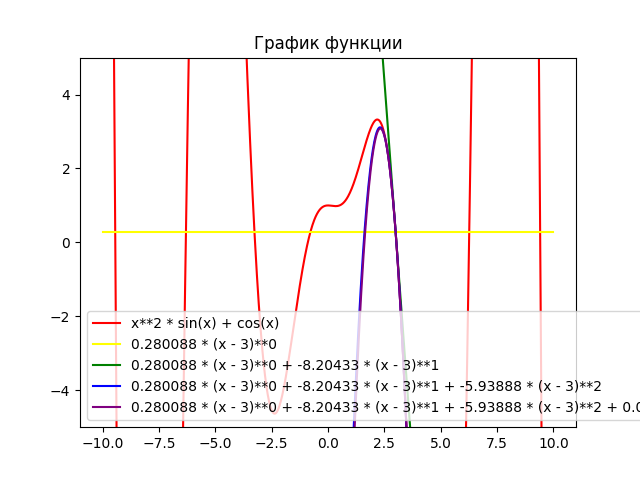
\includegraphics[scale=0.6]{plot.png} \end{center}
\textbf{* Разложения... Ну вы поняли)))}\subsection{Графики разностей}
\begin{center} 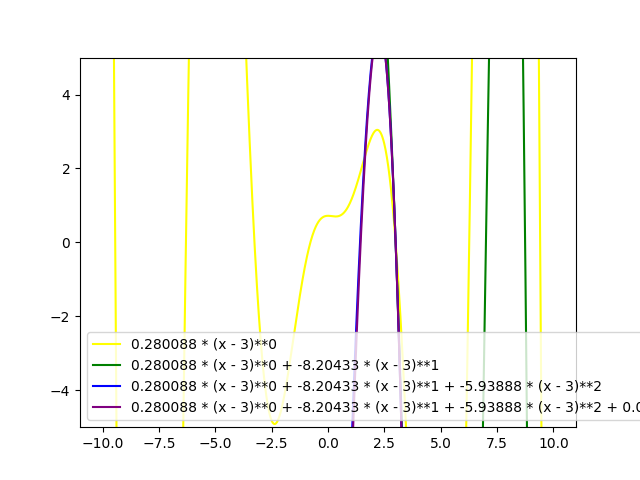
\includegraphics[scale=0.6]{difference.png} \end{center}
\section{Вывод}\begin{center} 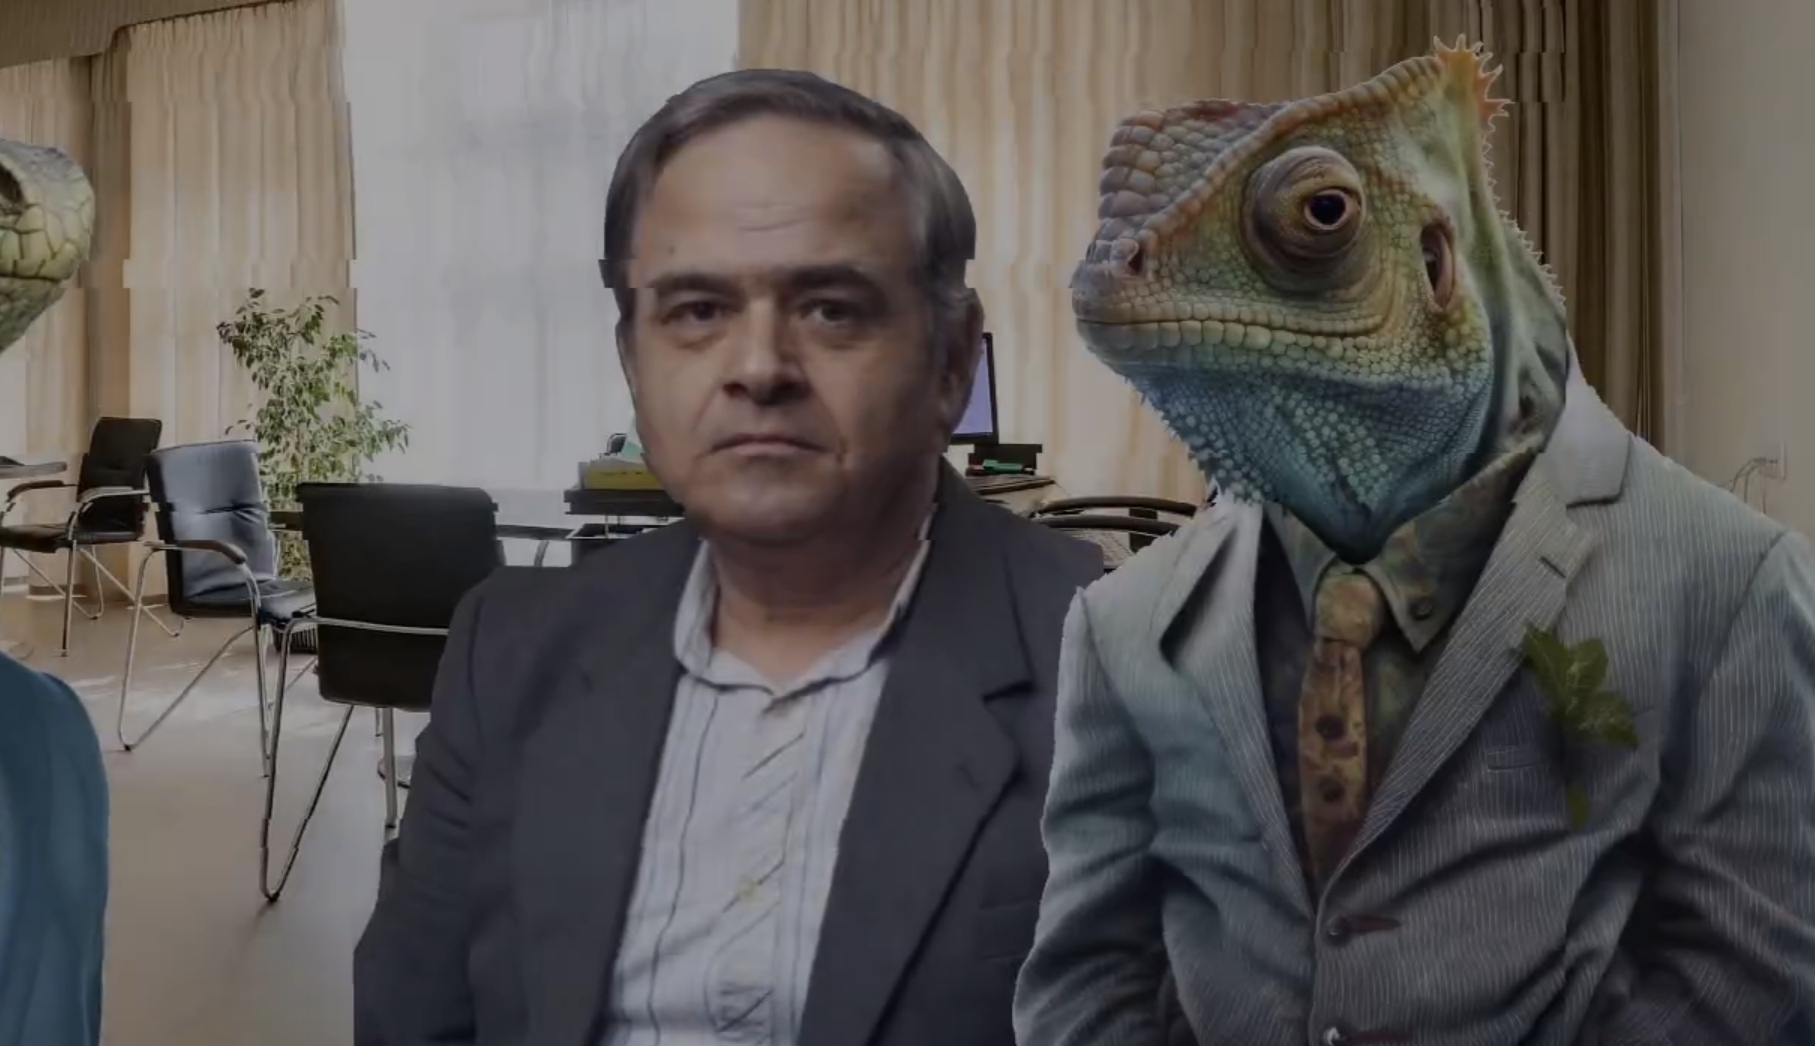
\includegraphics[scale=0.2]{Petrovich.jpg} \end{center}
\end{document}